\documentclass{beamer}
\mode<presentation>
{
  \usetheme{Warsaw}
  \definecolor{mcgarnet}{rgb}{0.38, 0, 0.08}
  \definecolor{mcgray}{rgb}{0.6, 0.6, 0.6}
  \setbeamercolor{structure}{fg=mcgarnet,bg=mcgray}
  %\setbeamercovered{transparent}
}


\usepackage[english]{babel}
\usepackage[latin1]{inputenc}
\usepackage{times}
\usepackage[T1]{fontenc}
\usepackage{tikz}
\usepackage{graphicx}
\usepackage{adjustbox}
\usepackage{fancyvrb}

\newcommand{\imagesource}[1]{{\centering\hfill\break\hbox{\scriptsize Image Source:\thinspace{\small\itshape #1}}\par}}

\title{Introduction to C++}


\author{Dr. Robert Lowe\\}

\institute[Maryville College] % (optional, but mostly needed)
{
  Division of Mathematics and Computer Science\\
  Maryville College
}

\date[]{}
\subject{CSC111 - Introduction to Computer Science I}

\pgfdeclareimage[height=0.5cm]{university-logo}{images/Maryville-College}
\logo{\pgfuseimage{university-logo}}



\AtBeginSection[]
{
  \begin{frame}<beamer>{Outline}
    \tableofcontents[currentsection]
  \end{frame}
}

\newcounter{reposteps}

\begin{document}

\begin{frame}
  \titlepage
\end{frame}

\begin{frame}{Outline}
  \tableofcontents
\end{frame}


% Structuring a talk is a difficult task and the following structure
% may not be suitable. Here are some rules that apply for this
% solution: 

% - Exactly two or three sections (other than the summary).
% - At *most* three subsections per section.
% - Talk about 30s to 2min per frame. So there should be between about
%   15 and 30 frames, all told.

% - A conference audience is likely to know very little of what you
%   are going to talk about. So *simplify*!
% - In a 20min talk, getting the main ideas across is hard
%   enough. Leave out details, even if it means being less precise than
%   you think necessary.
% - If you omit details that are vital to the proof/implementation,
%   just say so once. Everybody will be happy with that.

\section{Working with Git}
\begin{frame}{Your Repository}
\begin{enumerate}[<+->]
    \item Check your email. Look for an invite to a repository named:
        \newline{\tt cs1-fall2019-{\em username}}
    \item Accept the invitation.
    \item Look at the repository on GitHub.
        \newline\includegraphics[height=2cm]{images/cs1-repo}
    \item Log in to cs.maryvillecollege.edu via ssh.
    \item On GitHub, click ``Clone or download'' and select ``https''.
        \newline\includegraphics[height=3cm]{images/cs1-clone}
    \setcounter{reposteps}{\value{enumi}}
\end{enumerate}
\end{frame}

\begin{frame}{Your Repository (ctd.)}
\begin{enumerate}[<+->]
    \setcounter{enumi}{\value{reposteps}}
    \item Copy the https URL to your clipboard.
    \item Type the following command in your ssh shell (pasting the
    URL where specified)
        \newline{\tt git clone {\em <<Paste URL Here>>}}
    \item Change into your {\tt cs1-fall2019-{\em username}}
    directory.  
        \newline {\bf HINT}: Use tab completion!  Type {\tt cd cs1} and
    then press the tab key.  It saves time!
    \item Look around in your newly cloned repository.  This is where
    you will do all of your work!
\end{enumerate}
\end{frame}

\begin{frame}{Basic {\tt git} Commands}

Basic Pattern: {\tt git {\em command} {\em args}}
\begin{description}[<+->]
    \item[{\tt git clone {\em url}}] Clone a repository to your
        current directory.
    \item[{\tt git pull}] Pull changes from GitHub.  (Do this at the
        beginning of each class meeting!)
    \item[{\tt git add {\em filename}}] Add a file to the list of
        files tracked by git.
    \item[{\tt git add -A}] Add all untracked files to the git
        repository.
    \item[{\tt git commit -a}] Commit all changes to the local
        repository.  (Do this at the end of every major change.)
    \item[{\tt git push}] Push all changes to GitHub.  (Do this at the
        end of every work session.)
\end{description}
\end{frame}

\begin{frame}{Your Workflow}

Each time you sit down to work:
\begin{enumerate}[<+->]
    \item Login on MCCS via ssh.
    \item Change into your {\tt cs1-fall2019-{\em username}}
    directory.
    \item {\tt git pull}
    \item Do some rather taxing and stressful programming.
    \item Periodically (and at the end): {\tt git add -A}
    \item Periodically (and at the end): {\tt git commit -a}
    \item At the end of your work session: {\tt git push}
    \item Contemplate coding until the blessed hour arrives when you
    can resume your work.
\end{enumerate}
\end{frame}


\section{Introduction to Programming}
\begin{frame}{Anatomy of a Computer}
\begin{columns}
\column{0.5\textwidth}
    \begin{itemize}[<+->]
        \item A {\bf computer} is a device which executes programs.
        \item The most common computer architecture is the Von-Neumann
            Architecture.
        \item Program code and data are stored in the same memory.
        \item {\bf CPU} Executes very simple instructions.
        \item Collectively, the components of a computer are called its
            {\bf hardware}.
    \end{itemize}
\column{0.5\textwidth}
    \includegraphics[width=0.9\textwidth]{images/von-neumann}
    \begin{center}
        {\tiny\bf Von-Neumann Architecture}
    \end{center}
\end{columns}
\end{frame}

\begin{frame}{Program Representation \& Translation}
    \begin{itemize}[<+->]
        \item The text typed by a programmer is called {\bf source
            code}.
        \item The binary code executed by a computer is called 
            {\bf object code} or {\bf machine code}.
        \item In {\bf interpreted} languages an {\bf interpreter} directly
            executes source code.
        \item In {\bf compiled} languages a {\bf compiler} translates source
            code into object code.
            \newline\includegraphics[width=0.8\textwidth]{images/compiler}
    \end{itemize}
\end{frame}

\begin{frame}[fragile]{A Program - In Machine Code}
\begin{verbatim}
b8 04 00 00 00 bb 01 00 00 00 b9 25 10 40 00 ba
33 10 40 00 81 ea 25 10 40 00 cd 80 b8 01 00 00
00 31 db cd 80 68 65 6c 6c 6f 2c 20 77 6f 72 6c
64 0a 00 00
\end{verbatim}

\begin{itemize}[<+(1)->]
    \item What does this do?
    \item Really, even this needs to have a bit of a wrapper to turn
    it into binary.
    \item Change into your {\tt examples/01-Intro-C++} directory.
    \item {\tt cat prognum.S}
    \item {\tt as prognum.S -o prognum.o}
    \item {\tt ld prognum.o -o prognum}
    \item {\tt ./prognum}
\end{itemize}
\end{frame}

\begin{frame}[fragile]{A Program - In Assembly}
    \begin{columns}
    \column{0.5\textwidth}
    \begin{adjustbox}{max height=0.8\textheight, max width=0.95\textwidth}
    \begin{BVerbatim}
.text
.globl _start

_start:
            movl    $4, %eax
            movl    $1, %ebx
            movl    $msg, %ecx
            movl    $msgend, %edx
            sub     $msg, %edx
            int     $0x80

            movl    $1, %eax
            xorl    %ebx, %ebx
            int     $0x80
msg:    .string "hello, world\n"
msgend: .byte 0
    \end{BVerbatim}
    \end{adjustbox}

    \column{0.5\textwidth}
    \begin{itemize}[<+(1)->]
        \item Make sure you are in {\tt examples/01-Intro-C++}.
        \item {\tt cat hello.S}
        \item {\tt as hello.S -o hello.o}
        \item {\tt ld hello.o -o hello}
        \item {\tt ./hello}
    \end{itemize}
    \end{columns}
\end{frame}

\begin{frame}[fragile]{A Program - In Python}
    \begin{verbatim}
print "hello, world"
    \end{verbatim}

    \begin{itemize}[<+(1)->]
        \item Make sure you are in {\tt examples/01-Intro-C++}.
        \item {\tt cat hello.py}
        \item {\tt python hello.py}
    \end{itemize}
\end{frame}

\begin{frame}{Levels of Abstraction}
    \begin{columns}
        \column{0.6\textwidth}
        \begin{itemize}[<+->]
            \item (Too) Many programming languages exist.
            \item Each language is designed for some set of purposes.
            \item Usually, humans desire a fair degree of 
                {\bf abstraction}.
            \item A programming language's level of abstraction is the
                degree to which it hides details from the programmer.
        \end{itemize}

        \column{0.4\textwidth}
        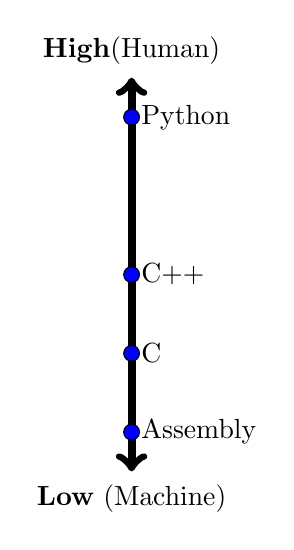
\begin{tikzpicture}
            \draw[line width=0.1cm,<->] 
              (0,1) node[below]{{\bf Low} (Machine)}
              -- (0,6) node[above]{{\bf High}(Human)};
            \uncover<+->{\draw[fill=blue] (0,1.5) circle (0.1cm)
                node[right]{Assembly};}
            \uncover<+->{\draw[fill=blue] (0,5.5) circle (0.1cm)
                node[right]{Python};}
            \uncover<+->{\draw[fill=blue] (0,2.5) circle(0.1cm)
                node[right]{C};}
            \uncover<+->{\draw[fill=blue] (0,3.5) circle(0.1cm)
                node[right]{C++};}
        \end{tikzpicture}
    \end{columns}
\end{frame}

\begin{frame}{The C++ Programming Language}
    \begin{columns}
        \column{0.6\textwidth}
        \begin{itemize}[<+(1)->]
            \item Created at Bell Labs by Bjarne Stroustrup as
                a successor to the C programming language.
            \item Adds Object Oriented Programming to C.
            \item Compiled, Mid-Level language.
            \item Ported to virtually all modern platforms.
            \item Low level access with high level facilities.
            \item You get to explore a bit of all worlds when learning
                C++!
        \end{itemize}

        \column{0.4\textwidth}
        \includegraphics[width=0.8\textwidth]{images/bjarne}
        \begin{center}
            \tiny
            Source: \url{https://en.wikipedia.org/wiki/Bjarne_Stroustrup}
        \end{center}
    \end{columns}
\end{frame}


\section{Our First C++ Program}
\begin{frame}{Creating The {\tt week2} Directory}
    \begin{enumerate}[<+->]
        \item Change to your {\tt $\sim$/cs1-fall2019-{\em username}}
            directory.
        \item {\tt cd labs}
        \item {\tt mkdir week2}
        \item {\tt cd week2}
    \end{enumerate}
\end{frame}

\begin{frame}[fragile]{Create {\tt hello.cpp}}

Using the text editor of your choice, enter the following into a file
titled {\tt hello.cpp}.

\begin{verbatim}
#include <iostream>

using namespace std;

int main()
{
    cout << "hello, world" << endl;
}
\end{verbatim}
\end{frame}

\begin{frame}{Compile {\tt hello.cpp}}
\begin{enumerate}[<+->]
    \item {\tt g++ hello.cpp -o hello}
    \item Correct any errors you may have encountered.
    \item Once it compiles error free, proceed.
    \item {\tt ./hello}
\end{enumerate}
\end{frame}

\begin{frame}{Push Your Work to GitHub}
\begin{enumerate}[<+->]
    \item {\tt git add hello.cpp}
    \item {\tt git commit hello.cpp -m 'Added hello.cpp'}
    \item {\tt git push}
    \item Go to your GitHub repository and verify that your file is in
    your {\tt labs/week2} folder.
\end{enumerate}
\end{frame}

\end{document}


